%======================================================================
\Q{Problem 1: Hazardous and safe zones of an antenna larger than a wavelength (the full method)}{\m{4}\m{3}\m{4}}
{\color{sub}\footnotesize \yr{\textbf{\texttt{81 Bh}}} solved in full \gap$\cdot$\gap \yr{74 Ma, \textbf{77 Ch}} (microwave oven) in the sibling table}

\begin{asked}{\textbf{\texttt{81 Bh}} \ [4+4]}
Approximate the hazardous and safe zone for BTS tower operating at 2600MHz with antenna size of 0.5 m. Explain, how non-radiating radiation is hazardous to the human body?
\end{asked}
{\color{sub}\footnotesize The second part is theory: $\S$7.2, ``how is non-radiating radiation hazardous''.}

\lead{Given}
\begin{itemize}
  \item $f = 2600$ MHz $= 2.6\times10^9$ Hz, antenna largest dimension $D = 0.5$ m,
    $c = 3\times10^8$ m/s.
\end{itemize}

\lead{Formulas}
\[ \lambda = \frac{c}{f}, \qquad R_1 = 0.62\sqrt{\frac{D^3}{\lambda}}, \qquad R_2 = \frac{2D^2}{\lambda} \]
{\color{sub}\footnotesize $R < R_1$ reactive near field, $R_1 < R < R_2$ radiating near field (Fresnel), $R > R_2$ far field. Valid when $D > \lambda$.}

\par\penalty0\Needspace{14\baselineskip}
\lead{Step-by-step}
{\renewcommand{\arraystretch}{2.0}%
\begin{tabularx}{\linewidth}{@{}L{0.5cm}L{3.3cm}L{6.2cm}X@{}}
\toprule
\hrow \thead{\#} & \thead{Quantity} & \thead{Substitution} & \thead{Value} \\
\midrule
1 & wavelength $\lambda$ & $\dfrac{3\times10^8}{2.6\times10^9}$ & $0.1154$ m \\
2 & validity check & $D = 0.5$ m vs $\lambda = 0.1154$ m & $D = 4.3\lambda > \lambda$ \checkmark \\
3 & $D^3/\lambda$ & $\dfrac{0.5^3}{0.1154} = \dfrac{0.125}{0.1154}$ & $1.0833$ m$^2$ \\
4 & $R_1$ & $0.62\sqrt{1.0833} = 0.62\times1.0408$ & $\mathbf{0.645\ m}$ \\
5 & $R_2$ & $\dfrac{2\times0.5^2}{0.1154} = \dfrac{0.5}{0.1154}$ & $\mathbf{4.33\ m}$ \\
\bottomrule
\end{tabularx}}
{\color{sub}\footnotesize Why step 2: the formulas describe an aperture larger than a wavelength. If $D < \lambda$ they must not be used (Problem 2).}

\par\penalty0\Needspace{12\baselineskip}
\lead{Final answer}
\begin{tabularx}{\linewidth}{@{}L{3.6cm}L{3.6cm}X@{}}
\toprule
\hrow \thead{Zone} & \thead{Distance from antenna} & \thead{Verdict} \\
\midrule
Reactive near field & $R < 0.645$ m & \textbf{hazardous} (stored-energy coupling) \\
Radiating near field & $0.645 < R < 4.33$ m & \textbf{hazardous} (full beam power, not yet spreading) \\
Far field & $R > 4.33$ m & \textbf{safe side}: power density falls as $1/R^2$ \\
\bottomrule
\end{tabularx}
\[ \boxed{\text{Hazardous zone: within } 4.33 \text{ m of the antenna} \qquad \text{Safe zone: beyond } 4.33 \text{ m}} \]
\par\penalty0\Needspace{11\baselineskip}
\lead{The zone figure, to scale}
\mbox{}\hfill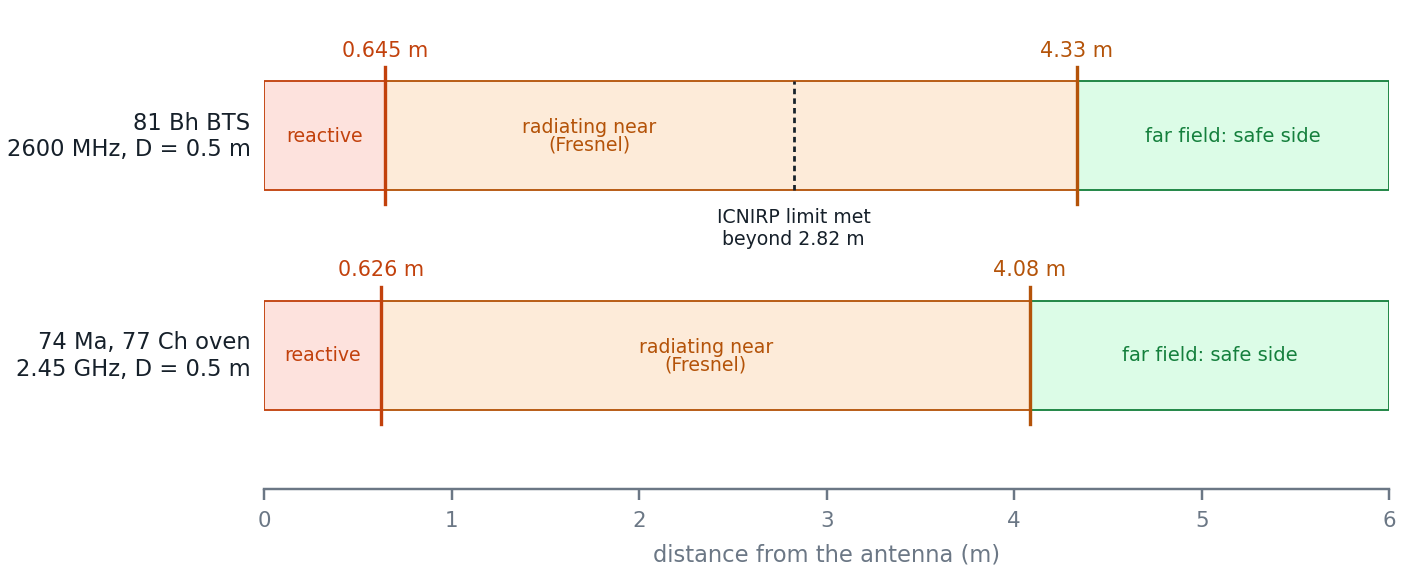
\includegraphics[width=0.80\textwidth]{figs/c7n_p1_zones.png}\hfill\mbox{}\par
{\color{sub}\footnotesize What ``approximate the zones'' and the oven's ``illustrate the radiation
fields'' want drawn: the three regions along the distance from the source, boundaries marked.
The dashed line is the ICNIRP compliance distance from the cross-check below. Generated by
\code{zonefig.py}, which checks every boundary against this page.}

\par\penalty0\Needspace{12\baselineskip}
\lead{Cross-check against the exposure limit \added{}}
\begin{itemize}
  \item The paper gives no power, so assume a typical sector: $P_t = 20$ W into a
    $G = 17$ dBi $= 50.1$ panel $\rightarrow$ EIRP $= 20\times50.1 = 1002$ W.
  \item ICNIRP 1998 public limit above 2 GHz: $S_{lim} = 10$ W/m$^2$ ($\S$7.4).
  \item Compliance distance $R = \sqrt{\dfrac{\text{EIRP}}{4\pi S_{lim}}} = \sqrt{\dfrac{1002}{4\pi\times10}} = \sqrt{7.98} = 2.82$ m
    (occupational limit 50 W/m$^2$: 1.26 m).
  \item At the far-field boundary $S = \dfrac{1002}{4\pi\times4.33^2} = 4.25$ W/m$^2$, under
    half the limit.
  \item So the zone answer (4.33 m) is the \textbf{more conservative} of the two: anyone kept
    beyond the far-field boundary is also within the limit. Every value: \code{ant.py}.
\end{itemize}

\par\penalty0\Needspace{14\baselineskip}
\lead{Sibling instances: same method, only the numbers change}
\begin{tabularx}{\linewidth}{@{}L{2.2cm}L{3.9cm}L{1.3cm}XL{0.9cm}@{}}
\toprule
\hrow \thead{Paper} & \thead{Given} & \thead{$\lambda$} & \thead{Reactive / Fresnel / far} & \thead{OK?} \\
\midrule
\textbf{\texttt{81 Bh}} (above) & BTS, 2600 MHz, $D = 0.5$ m & 0.1154 m & $< 0.645$ m / $0.645$ to $4.33$ m / $> 4.33$ m & yes \\
74 Ma, \textbf{77 Ch} & microwave oven, 2.45 GHz, $D = 0.5$ m (assumed, as the deck does) & 0.1224 m & $< 0.626$ m / $0.626$ to $4.08$ m / $> 4.08$ m & yes \\
\bottomrule
\end{tabularx}

\begin{asked}{74 Ma \ [4+4]}
What are the different types of electromagnetic radiation hazard? Illustrate radiation fields of a microwave oven.
\end{asked}
\begin{asked}{\textbf{77 Ch} \ [3+3]}
How are microwaves hazardous to humans? Define different radiation zones of a microwave oven.
\end{asked}
\begin{itemize}
  \item Oven working, step by step: $\lambda = 3\times10^8/2.45\times10^9 = 0.1224$ m;
    $D^3/\lambda = 0.125/0.1224 = 1.021$; $R_1 = 0.62\times1.010 = 0.626$ m;
    $R_2 = 0.5/0.1224 = 4.08$ m. The deck prints 0.6266 m and 4.085 m from the same numbers.
  \item Add the oven-specific point: the metal cavity and door mesh keep leakage below
    1 mW/cm$^2$ at 5 cm, so the zones apply to \textbf{leakage} only ($\S$7.1). Draw the zone
    figure with the oven at the source end.
\end{itemize}

\penalty0\vspace{2pt}

%======================================================================
\Q{Problem 2: Radiation fields of a small (quarter-wave) antenna, 900 MHz vs 1800 MHz}{\m{4}}
{\color{sub}\footnotesize \yr{\texttt{82 Ba}} \gap$\cdot$\gap solved separately because the Problem-1 formulas break down for $D < \lambda$}

\begin{asked}{\texttt{82 Ba} \ [4+2+2]}
Compare radiation fields around a mobile BTS operating at 900 MHz and 1800 MHz frequency bands with their quarter-wavelength antennas. Explain how microwave EMR becomes hazardous to humans; and mention its IEEE safety standard.
\end{asked}
{\color{sub}\footnotesize Parts two and three are theory: $\S$7.2 and $\S$7.4 (IEEE C95.1).}

\lead{Given}
\begin{itemize}
  \item $f_1 = 900$ MHz, $f_2 = 1800$ MHz, antenna length $D = \lambda/4$ at each frequency.
\end{itemize}

\lead{Method}
\begin{itemize}
  \item First apply the textbook formulas, as the examiner expects. With $D = \lambda/4$ they
    reduce to
    \[ R_1 = 0.62\sqrt{\frac{(\lambda/4)^3}{\lambda}} = \frac{0.62\,\lambda}{8} = 0.0775\lambda, \qquad R_2 = \frac{2(\lambda/4)^2}{\lambda} = \frac{\lambda}{8} = 0.125\lambda \]
  \item Then check validity: $D < \lambda$, and $R_2 = 0.125\lambda$ is inside
    $\lambda/2\pi = 0.159\lambda$, where the reactive field of any small antenna still
    dominates. So the ``far field'' of the formula is not a far field. Use the small-antenna
    boundaries \added{}: reactive out to $\lambda/2\pi$, far field beyond about $2\lambda$,
    a transition region between.
\end{itemize}

\par\penalty0\Needspace{16\baselineskip}
\lead{Step-by-step}
\begin{tabularx}{\linewidth}{@{}L{4.6cm}L{4.0cm}XX@{}}
\toprule
\hrow \thead{Quantity} & \thead{Formula} & \thead{900 MHz} & \thead{1800 MHz} \\
\midrule
wavelength & $\lambda = c/f$ & $0.3333$ m & $0.1667$ m \\
antenna length & $D = \lambda/4$ & $8.33$ cm & $4.17$ cm \\
textbook reactive boundary & $R_1 = 0.0775\lambda$ & $2.58$ cm & $1.29$ cm \\
textbook far-field boundary & $R_2 = 0.125\lambda$ & $4.17$ cm & $2.08$ cm \\
validity & $D > \lambda$? & no & no \\
\midrule
reactive near field (use) & $R < \lambda/2\pi$ & $R < 5.3$ cm & $R < 2.7$ cm \\
transition (radiating near) & $\lambda/2\pi$ to $2\lambda$ & $5.3$ to $66.7$ cm & $2.7$ to $33.3$ cm \\
far field (use) & $R > 2\lambda$ & $R > 0.67$ m & $R > 0.33$ m \\
\midrule
public limit, FCC & $f/1500$ or 1.0 mW/cm$^2$ & $0.6$ mW/cm$^2$ & $1.0$ mW/cm$^2$ \\
public limit, ICNIRP & $f/200$ W/m$^2$ & $4.5$ W/m$^2$ & $9$ W/m$^2$ \\
\bottomrule
\end{tabularx}

\par\penalty0\Needspace{12\baselineskip}
\lead{Final answer: the comparison}
\begin{itemize}
  \item \textbf{Every zone boundary scales with $\lambda$}, so at 1800 MHz each zone is
    \textbf{half} the size of the 900 MHz one:
    \[ \boxed{\text{far field beyond } 0.67 \text{ m at 900 MHz}, \quad 0.33 \text{ m at 1800 MHz}} \]
    \mbox{}\hfill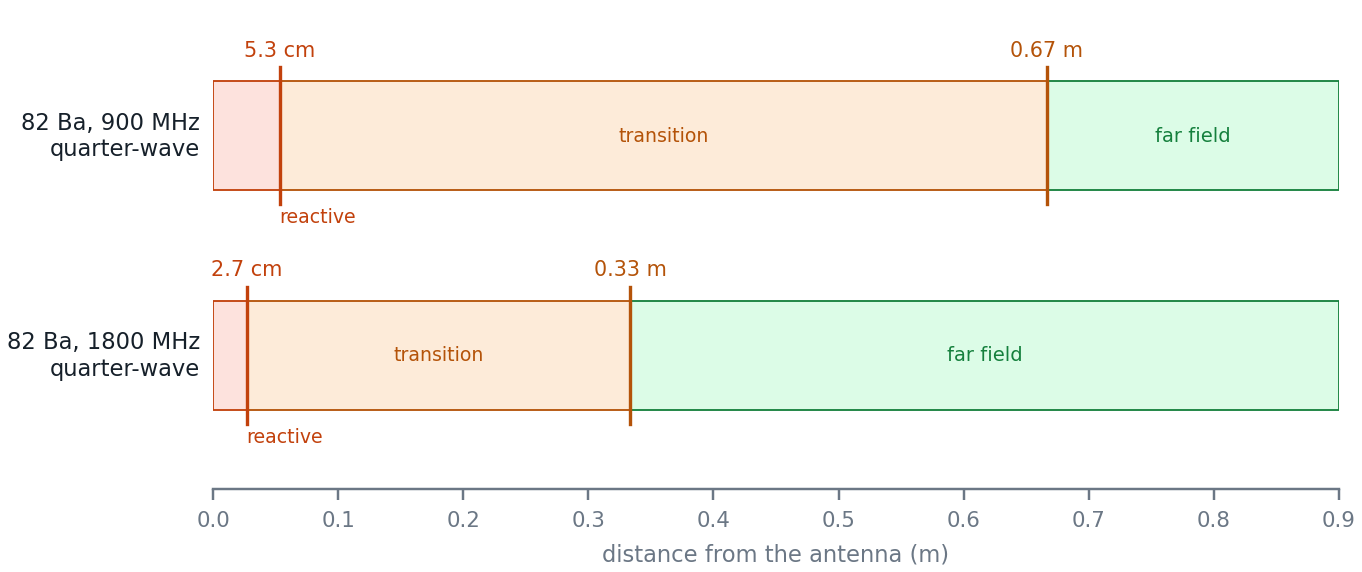
\includegraphics[width=0.74\linewidth]{figs/c7n_p2_zones.png}\hfill\mbox{}\par
    {\color{sub}\footnotesize The comparison drawn to one scale: every 1800 MHz boundary is half
    the 900 MHz one. From \code{zonefig.py}.}
  \item Both antennas are electrically small, so the near-field region is tiny: anyone more
    than a metre away is in the far field of either, and exposure there is set by power and
    distance ($S = P_tG/4\pi R^2$), not by zone.
  \item \textbf{900 MHz}: longer wavelength penetrates deeper into tissue (several cm) and is
    nearer the body-resonance region $\rightarrow$ \textbf{tighter} limit (0.6 mW/cm$^2$).
  \item \textbf{1800 MHz}: absorbed more superficially $\rightarrow$ limit relaxes to
    1.0 mW/cm$^2$. Higher path loss $\rightarrow$ smaller cells, more sites, lower power
    per site.
\end{itemize}
{\color{sub}\footnotesize The same break-down hits the deck's second example (150 MHz, $D = 0.5$ m, $\lambda = 2$ m): it prints reactive $< 0.155$ m and far field $> 0.25$ m, but $0.25$ m is inside $\lambda/2\pi = 0.32$ m. The small-antenna rule gives reactive $< 0.32$ m, far field $> 4$ m. The formulas cross over at $D = 0.28\lambda$ (\code{ant.py}).}
